\documentclass[10pt,landscape]{article}
\usepackage{xcolor}
\usepackage{multicol}
\usepackage{calc}
\usepackage{ifthen}
\usepackage[landscape]{geometry}
\usepackage{hyperref}
\hypersetup{
    colorlinks,
    linkcolor={red!50!black},
    citecolor={blue!50!black},
    urlcolor={blue!80!black}
}

\usepackage{graphicx}
\usepackage[export]{adjustbox}
\usepackage{enumitem}

\usepackage[defaultsans]{droidsans}
\renewcommand*\familydefault{\sfdefault} %% Only if the base font of the document is to be typewriter style
\usepackage[T1]{fontenc}


\usepackage{listings}
\usepackage[framemethod=TikZ]{mdframed}

\definecolor{bg}{gray}{0.96}
\definecolor{faded}{gray}{0.6}

\lstdefinestyle{commands}{
    backgroundcolor=\color{bg},
    basicstyle=\footnotesize,
    breakatwhitespace=false,
    breaklines=true,
    keepspaces=true,
    numbers=none,
    numbersep=5pt,
    showspaces=false,
    showstringspaces=false,
    showtabs=false,
    tabsize=2
}
\mdfdefinestyle{commands}{%
    backgroundcolor=bg,
    innertopmargin=4pt,
    middlelinewidth=1pt,
    outerlinewidth=1pt,
    outerlinecolor=white,
    innerleftmargin=5pt,
    innerrightmargin=5pt,
    leftmargin=-1pt,rightmargin=-1pt,
    skipabove=\topskip,
    skipbelow=\topskip,
    roundcorner=1pt,
    singleextra={\node[fill=white,anchor=west, xshift=10pt+1pt,font=\bfseries] at (O|-P) {\csname mdf@@codeheading\endcsname};},
}

\lstdefinestyle{examples}{
    backgroundcolor=\color{white},%
    numberstyle=\tiny\color{bg},
    basicstyle=\footnotesize,
    breakatwhitespace=false,
    breaklines=true,
    keepspaces=true,
    numbers=none,
    numbersep=5pt,
    showspaces=false,
    showstringspaces=false,
    showtabs=false,
    tabsize=2
}
\mdfdefinestyle{examples}{%
    backgroundcolor=white,
    innertopmargin=1pt,
    middlelinewidth=1pt,
    outerlinewidth=1pt,
    outerlinecolor=white,
    innerleftmargin=5pt,
    innerrightmargin=5pt,
    leftmargin=-1pt,rightmargin=-1pt,
    skipabove=\topskip,
    skipbelow=\topskip,
    roundcorner=1pt,
    singleextra={\node[fill=white,anchor=west, xshift=10pt+1pt] at (O|-P) {\csname mdf@@codeheading\endcsname};},
}


\makeatletter
\def\mdf@@codeheading{Code Listings}%new mdframed key:
\define@key{mdf}{title}{%
   \def\mdf@@codeheading{#1}
}

\lstnewenvironment{code}[2][]{%
  \lstset{#1}%
  \mdframed[style=commands,title={#2}]%
}{\endmdframed}


\lstnewenvironment{commands}[2][]{%
  \lstset{style=commands}%
  \lstset{#1}%
  \mdframed[style=commands,title={#2}]%
}{\endmdframed}

\lstnewenvironment{examples}[2][]{%
  \lstset{style=examples}%
  \lstset{#1}%
  \mdframed[style=examples,title={#2}]%
}{\endmdframed}




\lstset{style=commands}



% This sets page margins to .5 inch if using letter paper, and to 1cm
% if using A4 paper. (This probably isn't strictly necessary.)
% If using another size paper, use default 1cm margins.
\ifthenelse{\lengthtest { \paperwidth = 11in}}
{ \geometry{top=.5in,left=.5in,right=.5in,bottom=.5in} }
{\ifthenelse{ \lengthtest{ \paperwidth = 297mm}}
    {\geometry{top=1cm,left=1cm,right=1cm,bottom=1cm} }
    {\geometry{top=1cm,left=1cm,right=1cm,bottom=1cm} }
}

% Turn off header and footer
\pagestyle{empty}


% Redefine section commands to use less space
\makeatletter
\renewcommand{\section}{\@startsection{section}{1}{0mm}%
                                {-1ex plus -.5ex minus -.2ex}%
                                {0.5ex plus .2ex}%x
                                {\normalfont\large\bfseries}}
\renewcommand{\subsection}{\@startsection{subsection}{2}{0mm}%
                                {-1explus -.5ex minus -.2ex}%
                                {0.5ex plus .2ex}%
                                {\normalfont\normalsize\bfseries}}
\renewcommand{\subsubsection}{\@startsection{subsubsection}{3}{0mm}%
                                {-1ex plus -.5ex minus -.2ex}%
                                {1ex plus .2ex}%
                                {\normalfont\small\bfseries}}
\makeatother

% Define BibTeX command
\def\BibTeX{{\rm B\kern-.05em{\sc i\kern-.025em b}\kern-.08em
    T\kern-.1667em\lower.7ex\hbox{E}\kern-.125emX}}

% Don't print section numbers
\setcounter{secnumdepth}{0}


\setlength{\parindent}{0pt}
\setlength{\parskip}{0pt plus 0.5ex}


%\newcommand{\note}[1]{\medskip\textbf{Note:} {#1}\medskip}

\newcommand{\note}[2][Note]{
\begin{description}[font=\bfseries,leftmargin=1cm,style=sameline]
    \item [{#1}] {#2}
\end{description}
}

% -----------------------------------------------------------------------

\begin{document}

\raggedright
\footnotesize
\begin{multicols}{3}
\raggedcolumns


% multicol parameters
% These lengths are set only within the two main columns
%\setlength{\columnseprule}{0.25pt}
\setlength{\premulticols}{1pt}
\setlength{\postmulticols}{1pt}
\setlength{\multicolsep}{1em}
\setlength{\columnsep}{1em}

\includegraphics[width=2cm,valign=t]{res/yadtlogo}%
\hfill%
\begin{minipage}[t]{5cm}
{\Large{\textbf{yadt 1.8}}}\hfill
\textcolor{faded}{cheat sheet 0.3}\\[1em]
~\hfill\href{http://www.yadt-project.org/}{http://www.yadt-project.org/}
\end{minipage}


\section{Concept}

Using yadtshell you can orchestrate high level operations like updating
a group of hosts, as well as stopping and starting relevant and dependent
services in the correct order.
\medskip

The most important command is \verb+update+.\\
After running \verb+update+ successfully, all hosts are up-to-date and
all services are up and running.

\note{In case of a problem (i.e. a command terminates with exit~code~!=~0),
yadtshell stops immediately. Subsequent calls of the same command continue
where the previous call stopped.}

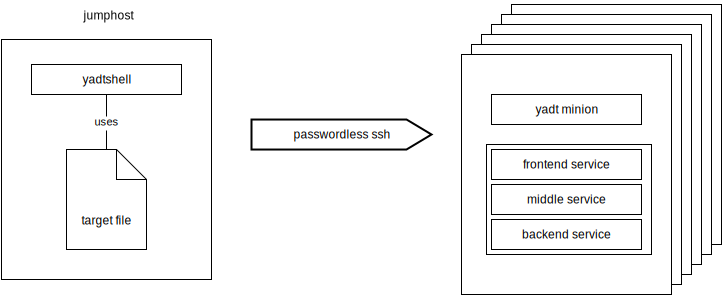
\includegraphics[width=\linewidth]{res/concept}

\note{It is required that the hosts are accessible
via passwordless ssh and provide a yadt minion (the counterpart to the yadtshell).}



\section{Component URIs}

\begin{commands}{component uris}
host://<hostname>
service://<hostname>/<name>
artefact://<hostname>/<name>/<version>
\end{commands}

\begin{examples}{Examples}
host://hostname
service://hostname/tomcat6
artefact://hostname/web-application/0:1.23
\end{examples}

\note{Components are \emph{always} host-specific.}

\begin{examples}{Brace Expression}
artefact://{hostname01|hostname03}/myapp
\end{examples}

\begin{examples}{Range Expression}
host://hostname0[1..3]
\end{examples}

\begin{examples}{Wildcards}
service://hostname/*
\end{examples}



\section{Host Configuration}

The yadt minion gets configured via \verb+*.yaml+ files in the
\verb+/etc/yadt.conf.d+ directory; they get merged in alphanumeric order.

\note{Indented blocks have to start with 4 blanks. Do \emph{not} use tabs.}

\begin{examples}[showspaces=true]{/etc/yadt.conf.d/my-services.yaml}
services:
    frontend:
        needs_services: [middleservice1]
        is_frontservice: true
    middleservice1:
        needs_services: [middleservice2]
\end{examples}

The service name must be equal to the corresponding name of the
service script (as found in \verb+/etc/init.d+).

\begin{description}[font=\bfseries,leftmargin=1cm,style=sameline]
    \item [is\_frontservice]
    is a marker for the status overview. The status
    (shown in percentage) of the target will be
    calculated by determining how many
    frontservices are running.
\item [needs\_services]
    the services that have to be running before
    starting this service (reverse for stopping)
\end{description}

The service definition may also contain a complete component URI as string,
which describes a service on another host, e.g.

\begin{examples}{need\_services}
needs_services: ['service://hostname/service']
\end{examples}

\note{This notation only allows the \emph{hostname},
not the full qualified domain name. Yadtshell extracts the hostname from
the fqdn as the string until the first dot.}

Please see the
\href{https://github.com/yadt/yadtshell/wiki/Host-Configuration}{host configuration section}
of the \href{https://github.com/yadt/yadtshell/wiki}{yadtshell wiki}
for more information.



\section{Target Configuration}

yadtshell uses a yaml file named
\verb+target+ in the current working directory to define a yadt target (set of hosts), e.g.

\begin{examples}{./target}
hosts:
- hostname1.spam.eggs
- hostname2.spam.eggs
- hostname*.spammy.eggs
- hostname0[1..3].foo.bar
\end{examples}

It is possible to group your hosts within a target:

\begin{examples}{./target}
hosts:
- hostname1.spam.eggs hostname2.spam.eggs
- hostname3.foo.bar hostname4.foo.bar
\end{examples}

This will change the way the hosts will be displayed.

%\vfill\columnbreak


%\section{view (file)}
%
%If you have a lot of hosts in a target you can use a yaml-file
%called view to configure the rendering of the status overview.
%Place the view file together with the target file in the current
%working directory.
%
%\begin{lstlisting}
%info-view: [matrix, color]
%\end{lstlisting}
%
%\begin{description}[font=\bfseries,leftmargin=1.5cm,style=sameline]
%    \item [matrix]  show status information in matrix
%    \item[color]    display status in color
%    \item[maxcols]  maximum number of columns
%    \item[3cols]    use three columns
%\end{description}
%
%
%\vfill\columnbreak



\section{Using the yadtshell}

\begin{commands}{start yadtshell}
> init-yadtshell
\end{commands}

\begin{itemize}
\item activates autocompletion for component uris,
\item allows to omit \verb#yadtshell# when executing yadtshell commands.
\end{itemize}

To restore your shell environment you can use \verb#CTRL+D# or

\begin{commands}{stop yadtshell}
> deactivate
\end{commands}


\newpage

\section{Yadtshell Commands}

Use the \verb#yadtshell# command if you prefer to execute yadtshell commands
without entering the yadtshell itself:
\begin{commands}{general usage}
> yadtshell [options] <command> [<uri> ...]
\end{commands}

\begin{description}[font=\bfseries,leftmargin=1.5cm,style=sameline]
    \item [-v]       verbose
    \item [--dryrun] no actions executed (just logging)
    \item [-n]       same as dryrun
\end{description}



\subsection{Status Information}

To retrieve the status of all services and artefact versions from the current
target use:
\begin{commands}{fetch status}
> status
\end{commands}

This will also perform \verb+info+, which displays a summary of all
services for each host within the current target:
\begin{commands}{show status}
> info [--full]
\end{commands}

\begin{description}[font=\bfseries,leftmargin=1.5cm,style=sameline]
    \item [--full]     shows complete information (artefacts of hosts, etc.)
\end{description}

To display low-level data of components (in yaml format) use
\begin{commands}{dump json data}
> dump [uri-query0 [uri-query1 ...]]
\end{commands}

additional arguments for \verb+dump+:
\begin{description}[font=\bfseries,leftmargin=1.5cm,style=sameline]
    \item [--attribute]
    \item [--show-pending-updates]
    \item [--show-current-artefacts]
\end{description}

\begin{examples}{dump raw data of all services}
> dump service://
\end{examples}

\note{The output of info and dump is generated using cached data.}



%\vfill\columnbreak
\subsection{Hosts}

To prevent others from executing commands on a host it is possible to lock the host:
\begin{commands}{lock host}
> lock -m "message" [--force] <host_uri> [...]
\end{commands}

afterwards commands can only be executed
\begin{itemize}
\item by you,
\item from the current target directory
\item on the current host.
\end{itemize}

\begin{examples}{lock hostname01}
> lock -m "I need this" host://hostname01
\end{examples}

\begin{examples}{hijacking a locked host}
> lock -m "hijacking" --force host://*
\end{examples}

\note{The message should reflect the reason why you are doing what you are doing and
include your name as well.}

\begin{examples}{with message}
> lock -m "updating host [Michael]" host://hostname31
\end{examples}

To release a lock use:
\begin{commands}{unlock host}
> unlock <host_uri> [<host_uri] ...]
\end{commands}

\begin{examples}{release all your locks on all hosts}
> unlock host://*
\end{examples}



%\vfill\columnbreak
\subsection{Services}

To start a service, regarding its dependencies, use:
\begin{commands}{start service}
> start <service_uri> [<service_uri> ...]
\end{commands}

\begin{examples}{start all services}
> start service://*
\end{examples}

To stop a service and all services depending on the service:
\begin{commands}{stop service}
> stop <service_uri> [<service_uri> ...]
\end{commands}

\note{When stopping a service, all services depending on this service will be
stopped as well. But starting the service will \emph{not} start the services
depending on the service again.}


If a service is currently out of order you can ignore the state of a service
(e.g. assume all operations on that service are successful):
\begin{commands}{ignore service}
> ignore -m "message" <service_uri> [...]
\end{commands}

\begin{examples}{nagios server down, so ignore}
> ignore -m "nagios server is down" service://*/nagios
\end{examples}

To unignore services on host use:
\begin{commands}{unignore service}
> unignore <service_uri> [...]
\end{commands}



%\vfill\columnbreak
\subsection{Artefacts}

To install updates (if there are any) and stop/start the defined services use:
\begin{commands}{update target}
> update [<host_uri> ...] [-p <number>]
\end{commands}


If you only want to update artefacts without restarting services,
use \verb+updateartefact+. Take care when using this command:
it is ignoring all service dependencies.
\begin{commands}{updateartefact}
> updateartefact <artefact_uri> [...]
\end{commands}



\begin{minipage}[b]{5cm}
~\hfill\href{https://github.com/yadt/yadtshell/wiki}{yadtshell wiki} at github

~\hfill\href{http://www.yadt-project.org/}{http://www.yadt-project.org/}
\end{minipage}%
\hfill%
\includegraphics[width=2cm,valign=b]{res/yadtlogo}%

\end{multicols}
\end{document}
